\documentclass[10pt,a4paper,onecolumn]{article}
\usepackage{marginnote}
\usepackage{graphicx}
\usepackage{xcolor}
\usepackage{authblk,etoolbox}
\usepackage{titlesec}
\usepackage{calc}
\usepackage{tikz}
\usepackage{hyperref}
\hypersetup{colorlinks,breaklinks,
            urlcolor=[rgb]{0.0, 0.5, 1.0},
            linkcolor=[rgb]{0.0, 0.5, 1.0}}
\usepackage{caption}
\usepackage{tcolorbox}
\usepackage{amssymb,amsmath}
\usepackage{ifxetex,ifluatex}
\usepackage{seqsplit}
\usepackage{xstring}

\usepackage{float}
\let\origfigure\figure
\let\endorigfigure\endfigure
\renewenvironment{figure}[1][2] {
    \expandafter\origfigure\expandafter[H]
} {
    \endorigfigure
}

\usepackage{fixltx2e} % provides \textsubscript
\usepackage[
  backend=biber,
%  style=alphabetic,
%  citestyle=numeric
]{biblatex}
\bibliography{paper.bib}

% --- Splitting \texttt --------------------------------------------------

\let\textttOrig=\texttt
\def\texttt#1{\expandafter\textttOrig{\seqsplit{#1}}}
\renewcommand{\seqinsert}{\ifmmode
  \allowbreak
  \else\penalty6000\hspace{0pt plus 0.02em}\fi}


% --- Pandoc does not distinguish between links like [foo](bar) and
% --- [foo](foo) -- a simplistic Markdown model.  However, this is
% --- wrong:  in links like [foo](foo) the text is the url, and must
% --- be split correspondingly.
% --- Here we detect links \href{foo}{foo}, and also links starting
% --- with https://doi.org, and use path-like splitting (but not
% --- escaping!) with these links.
% --- Another vile thing pandoc does is the different escaping of
% --- foo and bar.  This may confound our detection.
% --- This problem we do not try to solve at present, with the exception
% --- of doi-like urls, which we detect correctly.


\makeatletter
\let\href@Orig=\href
\def\href@Urllike#1#2{\href@Orig{#1}{\begingroup
    \def\Url@String{#2}\Url@FormatString
    \endgroup}}
\def\href@Notdoi#1#2{\def\tempa{#1}\def\tempb{#2}%
  \ifx\tempa\tempb\relax\href@Urllike{#1}{#2}\else
  \href@Orig{#1}{#2}\fi}
\def\href#1#2{%
  \IfBeginWith{#1}{https://doi.org}%
  {\href@Urllike{#1}{#2}}{\href@Notdoi{#1}{#2}}}
\makeatother

\newlength{\cslhangindent}
\setlength{\cslhangindent}{1.5em}
\newlength{\csllabelwidth}
\setlength{\csllabelwidth}{3em}
\newenvironment{CSLReferences}[3] % #1 hanging-ident, #2 entry spacing
 {% don't indent paragraphs
  \setlength{\parindent}{0pt}
  % turn on hanging indent if param 1 is 1
  \ifodd #1 \everypar{\setlength{\hangindent}{\cslhangindent}}\ignorespaces\fi
  % set entry spacing
  \ifnum #2 > 0
  \setlength{\parskip}{#2\baselineskip}
  \fi
 }%
 {}
\usepackage{calc}
\newcommand{\CSLBlock}[1]{#1\hfill\break}
\newcommand{\CSLLeftMargin}[1]{\parbox[t]{\csllabelwidth}{#1}}
\newcommand{\CSLRightInline}[1]{\parbox[t]{\linewidth - \csllabelwidth}{#1}}
\newcommand{\CSLIndent}[1]{\hspace{\cslhangindent}#1}

% --- Page layout -------------------------------------------------------------
\usepackage[top=3.5cm, bottom=3cm, right=1.5cm, left=1.0cm,
            headheight=2.2cm, reversemp, includemp, marginparwidth=4.5cm]{geometry}

% --- Default font ------------------------------------------------------------
% \renewcommand\familydefault{\sfdefault}

% --- Style -------------------------------------------------------------------
\renewcommand{\bibfont}{\small \sffamily}
\renewcommand{\captionfont}{\small\sffamily}
\renewcommand{\captionlabelfont}{\bfseries}

% --- Section/SubSection/SubSubSection ----------------------------------------
\titleformat{\section}
  {\normalfont\sffamily\Large\bfseries}
  {}{0pt}{}
\titleformat{\subsection}
  {\normalfont\sffamily\large\bfseries}
  {}{0pt}{}
\titleformat{\subsubsection}
  {\normalfont\sffamily\bfseries}
  {}{0pt}{}
\titleformat*{\paragraph}
  {\sffamily\normalsize}


% --- Header / Footer ---------------------------------------------------------
\usepackage{fancyhdr}
\pagestyle{fancy}
\fancyhf{}
%\renewcommand{\headrulewidth}{0.50pt}
\renewcommand{\headrulewidth}{0pt}
\fancyhead[L]{\hspace{-0.75cm}\includegraphics[width=5.5cm]{}}
\fancyhead[C]{}
\fancyhead[R]{}
\renewcommand{\footrulewidth}{0.25pt}

\fancyfoot[L]{\parbox[t]{0.98\headwidth}{\footnotesize{\sffamily , (). ShOpt.jl
\textbar{} A Julia Library for Empirical Point Spread Function
Characterization of JWST NIRCam
Data. \textit{}, (), . \url{https://doi.org/}}}}


\fancyfoot[R]{\sffamily \thepage}
\makeatletter
\let\ps@plain\ps@fancy
\fancyheadoffset[L]{4.5cm}
\fancyfootoffset[L]{4.5cm}

% --- Macros ---------

\definecolor{linky}{rgb}{0.0, 0.5, 1.0}

\newtcolorbox{repobox}
   {colback=red, colframe=red!75!black,
     boxrule=0.5pt, arc=2pt, left=6pt, right=6pt, top=3pt, bottom=3pt}

\newcommand{\ExternalLink}{%
   \tikz[x=1.2ex, y=1.2ex, baseline=-0.05ex]{%
       \begin{scope}[x=1ex, y=1ex]
           \clip (-0.1,-0.1)
               --++ (-0, 1.2)
               --++ (0.6, 0)
               --++ (0, -0.6)
               --++ (0.6, 0)
               --++ (0, -1);
           \path[draw,
               line width = 0.5,
               rounded corners=0.5]
               (0,0) rectangle (1,1);
       \end{scope}
       \path[draw, line width = 0.5] (0.5, 0.5)
           -- (1, 1);
       \path[draw, line width = 0.5] (0.6, 1)
           -- (1, 1) -- (1, 0.6);
       }
   }

% --- Title / Authors ---------------------------------------------------------
% patch \maketitle so that it doesn't center
\patchcmd{\@maketitle}{center}{flushleft}{}{}
\patchcmd{\@maketitle}{center}{flushleft}{}{}
% patch \maketitle so that the font size for the title is normal
\patchcmd{\@maketitle}{\LARGE}{\LARGE\sffamily}{}{}
% patch the patch by authblk so that the author block is flush left
\def\maketitle{{%
  \renewenvironment{tabular}[2][]
    {\begin{flushleft}}
    {\end{flushleft}}
  \AB@maketitle}}
\makeatletter
\renewcommand\AB@affilsepx{ \protect\Affilfont}
%\renewcommand\AB@affilnote[1]{{\bfseries #1}\hspace{2pt}}
\renewcommand\AB@affilnote[1]{{\bfseries #1}\hspace{3pt}}
\renewcommand{\affil}[2][]%
   {\newaffiltrue\let\AB@blk@and\AB@pand
      \if\relax#1\relax\def\AB@note{\AB@thenote}\else\def\AB@note{#1}%
        \setcounter{Maxaffil}{0}\fi
        \begingroup
        \let\href=\href@Orig
        \let\texttt=\textttOrig
        \let\protect\@unexpandable@protect
        \def\thanks{\protect\thanks}\def\footnote{\protect\footnote}%
        \@temptokena=\expandafter{\AB@authors}%
        {\def\\{\protect\\\protect\Affilfont}\xdef\AB@temp{#2}}%
         \xdef\AB@authors{\the\@temptokena\AB@las\AB@au@str
         \protect\\[\affilsep]\protect\Affilfont\AB@temp}%
         \gdef\AB@las{}\gdef\AB@au@str{}%
        {\def\\{, \ignorespaces}\xdef\AB@temp{#2}}%
        \@temptokena=\expandafter{\AB@affillist}%
        \xdef\AB@affillist{\the\@temptokena \AB@affilsep
          \AB@affilnote{\AB@note}\protect\Affilfont\AB@temp}%
      \endgroup
       \let\AB@affilsep\AB@affilsepx
}
\makeatother
\renewcommand\Authfont{\sffamily\bfseries}
\renewcommand\Affilfont{\sffamily\small\mdseries}
\setlength{\affilsep}{1em}


\ifnum 0\ifxetex 1\fi\ifluatex 1\fi=0 % if pdftex
  \usepackage[T1]{fontenc}
  \usepackage[utf8]{inputenc}

\else % if luatex or xelatex
  \ifxetex
    \usepackage{mathspec}
  \else
    \usepackage{fontspec}
  \fi
  \defaultfontfeatures{Ligatures=TeX,Scale=MatchLowercase}

\fi
% use upquote if available, for straight quotes in verbatim environments
\IfFileExists{upquote.sty}{\usepackage{upquote}}{}
% use microtype if available
\IfFileExists{microtype.sty}{%
\usepackage{microtype}
\UseMicrotypeSet[protrusion]{basicmath} % disable protrusion for tt fonts
}{}

\usepackage{hyperref}
\hypersetup{unicode=true,
            pdftitle={ShOpt.jl \textbar{} A Julia Library for Empirical Point Spread Function Characterization of JWST NIRCam Data},
            pdfborder={0 0 0},
            breaklinks=true}
\urlstyle{same}  % don't use monospace font for urls
\usepackage{color}
\usepackage{fancyvrb}
\newcommand{\VerbBar}{|}
\newcommand{\VERB}{\Verb[commandchars=\\\{\}]}
\DefineVerbatimEnvironment{Highlighting}{Verbatim}{commandchars=\\\{\}}
% Add ',fontsize=\small' for more characters per line
\newenvironment{Shaded}{}{}
\newcommand{\AlertTok}[1]{\textcolor[rgb]{1.00,0.00,0.00}{\textbf{#1}}}
\newcommand{\AnnotationTok}[1]{\textcolor[rgb]{0.38,0.63,0.69}{\textbf{\textit{#1}}}}
\newcommand{\AttributeTok}[1]{\textcolor[rgb]{0.49,0.56,0.16}{#1}}
\newcommand{\BaseNTok}[1]{\textcolor[rgb]{0.25,0.63,0.44}{#1}}
\newcommand{\BuiltInTok}[1]{#1}
\newcommand{\CharTok}[1]{\textcolor[rgb]{0.25,0.44,0.63}{#1}}
\newcommand{\CommentTok}[1]{\textcolor[rgb]{0.38,0.63,0.69}{\textit{#1}}}
\newcommand{\CommentVarTok}[1]{\textcolor[rgb]{0.38,0.63,0.69}{\textbf{\textit{#1}}}}
\newcommand{\ConstantTok}[1]{\textcolor[rgb]{0.53,0.00,0.00}{#1}}
\newcommand{\ControlFlowTok}[1]{\textcolor[rgb]{0.00,0.44,0.13}{\textbf{#1}}}
\newcommand{\DataTypeTok}[1]{\textcolor[rgb]{0.56,0.13,0.00}{#1}}
\newcommand{\DecValTok}[1]{\textcolor[rgb]{0.25,0.63,0.44}{#1}}
\newcommand{\DocumentationTok}[1]{\textcolor[rgb]{0.73,0.13,0.13}{\textit{#1}}}
\newcommand{\ErrorTok}[1]{\textcolor[rgb]{1.00,0.00,0.00}{\textbf{#1}}}
\newcommand{\ExtensionTok}[1]{#1}
\newcommand{\FloatTok}[1]{\textcolor[rgb]{0.25,0.63,0.44}{#1}}
\newcommand{\FunctionTok}[1]{\textcolor[rgb]{0.02,0.16,0.49}{#1}}
\newcommand{\ImportTok}[1]{#1}
\newcommand{\InformationTok}[1]{\textcolor[rgb]{0.38,0.63,0.69}{\textbf{\textit{#1}}}}
\newcommand{\KeywordTok}[1]{\textcolor[rgb]{0.00,0.44,0.13}{\textbf{#1}}}
\newcommand{\NormalTok}[1]{#1}
\newcommand{\OperatorTok}[1]{\textcolor[rgb]{0.40,0.40,0.40}{#1}}
\newcommand{\OtherTok}[1]{\textcolor[rgb]{0.00,0.44,0.13}{#1}}
\newcommand{\PreprocessorTok}[1]{\textcolor[rgb]{0.74,0.48,0.00}{#1}}
\newcommand{\RegionMarkerTok}[1]{#1}
\newcommand{\SpecialCharTok}[1]{\textcolor[rgb]{0.25,0.44,0.63}{#1}}
\newcommand{\SpecialStringTok}[1]{\textcolor[rgb]{0.73,0.40,0.53}{#1}}
\newcommand{\StringTok}[1]{\textcolor[rgb]{0.25,0.44,0.63}{#1}}
\newcommand{\VariableTok}[1]{\textcolor[rgb]{0.10,0.09,0.49}{#1}}
\newcommand{\VerbatimStringTok}[1]{\textcolor[rgb]{0.25,0.44,0.63}{#1}}
\newcommand{\WarningTok}[1]{\textcolor[rgb]{0.38,0.63,0.69}{\textbf{\textit{#1}}}}

% --- We redefined \texttt, but in sections and captions we want the
% --- old definition
\let\addcontentslineOrig=\addcontentsline
\def\addcontentsline#1#2#3{\bgroup
  \let\texttt=\textttOrig\addcontentslineOrig{#1}{#2}{#3}\egroup}
\let\markbothOrig\markboth
\def\markboth#1#2{\bgroup
  \let\texttt=\textttOrig\markbothOrig{#1}{#2}\egroup}
\let\markrightOrig\markright
\def\markright#1{\bgroup
  \let\texttt=\textttOrig\markrightOrig{#1}\egroup}


\usepackage{graphicx,grffile}
\makeatletter
\def\maxwidth{\ifdim\Gin@nat@width>\linewidth\linewidth\else\Gin@nat@width\fi}
\def\maxheight{\ifdim\Gin@nat@height>\textheight\textheight\else\Gin@nat@height\fi}
\makeatother
% Scale images if necessary, so that they will not overflow the page
% margins by default, and it is still possible to overwrite the defaults
% using explicit options in \includegraphics[width, height, ...]{}
\setkeys{Gin}{width=\maxwidth,height=\maxheight,keepaspectratio}
\IfFileExists{parskip.sty}{%
\usepackage{parskip}
}{% else
\setlength{\parindent}{0pt}
\setlength{\parskip}{6pt plus 2pt minus 1pt}
}
\setlength{\emergencystretch}{3em}  % prevent overfull lines
\providecommand{\tightlist}{%
  \setlength{\itemsep}{0pt}\setlength{\parskip}{0pt}}
\setcounter{secnumdepth}{0}
% Redefines (sub)paragraphs to behave more like sections
\ifx\paragraph\undefined\else
\let\oldparagraph\paragraph
\renewcommand{\paragraph}[1]{\oldparagraph{#1}\mbox{}}
\fi
\ifx\subparagraph\undefined\else
\let\oldsubparagraph\subparagraph
\renewcommand{\subparagraph}[1]{\oldsubparagraph{#1}\mbox{}}
\fi

\title{ShOpt.jl \textbar{} A Julia Library for Empirical Point Spread
Function Characterization of JWST NIRCam Data}

        \author[1]{Edward Berman}
          \author[1]{Jacqueline McCleary}
    
      \affil[1]{Northeastern University, USA}
  \date{\vspace{-5ex}}

\begin{document}
\maketitle

\marginpar{
  \sffamily\small

  {\bfseries DOI:} \href{https://doi.org/}{\color{linky}{}}

  \vspace{2mm}

  {\bfseries Software}
  \begin{itemize}
    \setlength\itemsep{0em}
    \item \href{}{\color{linky}{Review}} \ExternalLink
    \item \href{}{\color{linky}{Repository}} \ExternalLink
    \item \href{}{\color{linky}{Archive}} \ExternalLink
  \end{itemize}

  \vspace{2mm}

  {\bfseries Submitted:} \\
  {\bfseries Published:} 

  \vspace{2mm}
  {\bfseries License}\\
  Authors of papers retain copyright and release the work under a Creative Commons Attribution 4.0 International License (\href{https://creativecommons.org/licenses/by/4.0/}{\color{linky}{CC BY 4.0}}).
}

\hypertarget{summary}{%
\section{Summary}\label{summary}}

\hypertarget{introduction}{%
\subsection{Introduction}\label{introduction}}

When astronomers image the night sky, the path of the incoming light has
been altered by diffraction, optical aberrations, atmospheric
turbulence, and telescope jitter. These effects are summarized in the
image's point spread function (PSF), a mathematical model that describes
the response of an optical system to an idealized point of light.
Because the PSF can resemble or obscure the signal of interest, it must
be carefully modeled to extract the maximum amount of information from
an observation. Failing to do so can lead to inaccuracies in positions,
sizes, and shapes of targets like galaxies.

The goal of PSF characterization is to be able to point to any position
on your camera and predict what the distortion looks like. Once we have
a model that can do this well, we can deconvolve the PSF to produce
images free of distortion.

The PSF characterization methods used by astronomers fall into two main
classes: forward-modeling approaches, which use physical optics
propagation based on models of the optical array, and empirical
approaches, which use stars as fixed points to model and interpolate the
PSF across the rest of the image. (Stars are essentially point sources
before their light passes through the atmosphere and telescope, so the
shape and size of their surface brightness profiles axiomatically define
the PSF at that location.) Empirical PSF characterization proceeds by
first cataloging the observed stars, separating the catalog into
validation and training samples, and interpolating the training stars
across the field of view of the camera. We use the term vignets to
describe the image stamps containing stars that make up the catalog.
After training, the PSF model can be validated by comparing the reserved
stars to the PSF model's prediction.

Shear Optimization with \texttt{ShOpt.jl} introduces modern techniques
for empirical PSF characterization across the field of view that are
tailored to James Webb Space Telescope (JWST) imaging. ShOpt has two
modes of operation: approximating stars with analytic profiles, and a
more realistic pixel-level representation.

\hypertarget{analytic-profile-mode}{%
\subsection{Analytic profile mode}\label{analytic-profile-mode}}

A rough idea of the size and shape of the PSF can be obtained by fitting
stars with analytic profiles. We adopt a multivariate Gaussian profile
because it is computationally cheap to fit to an image. That is, it is
easy to differentiate and doesn't involve any numeric integration or
other costly steps to calculate. Fitting other common models, such as a
Kolmogorov profile, involves numeric integration and thus take much
longer to fit. Moreover, the JWST point spread function is very
``spikey'' (cf.~Figure 1). As a result, analytic profiles are limited in
their ability to model the point spread function anyway, making the
usual advantages of a more expensive analytic profile moot.

\begin{figure}
\centering
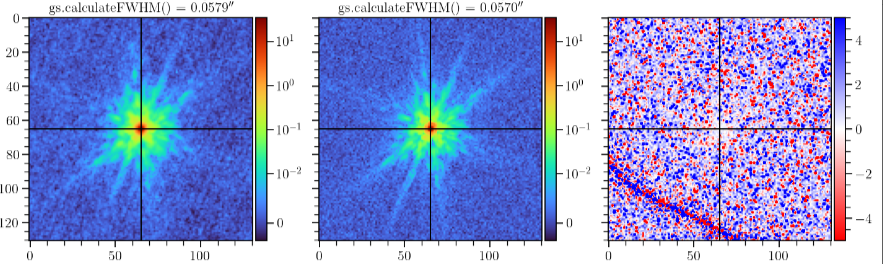
\includegraphics{spikey.png}
\caption{The plot on the left shows the average cutout of all of the
stars in a supplied catalog. Likewise, plot in the middle shows the
average point spread function model. The plot on the right shows the
average normalized error between the observed star cutouts and the point
spread function model.}
\end{figure}

Our multivariate gaussian is parameterized by three variables,
\([s, g_1, g_2]\), where \(s\) corresponds to size and \(g_1 , g_2\)
correspond to shear. A shear matrix has the form \[\begin{pmatrix}
1 + g_1 & g_2 \\
g_2 & 1 - g_1
\end{pmatrix}
\]. Given a point \([u, v]\), we obtain coordinates \([u' , v']\) by
applying a shear and then a scaling by
\(\frac{s}{\sqrt{1 - g_1^2 - g_2^2}}\). Then, we choose
\(f(r) := Ae^{-r^2}\) to complete our fit, where \(A\) makes the fit sum
to unity over the cutout of our star. After we fit this function to our
stars with \texttt{Optim.jl} (Mogensen and Riseth 2018) and
\texttt{ForwardDiff.jl} (Revels, Lubin, and Papamarkou 2016), we
interpolate the parameters across the field of view according to
position. Essentially, each star is a datapoint, and the three variables
are treated as polynomials in focal plane coordinates \((u,v)\) of
degree \(n\), where \(n\) is supplied by the user. The focal plain
refers to the set of points where an image appears to be in perfect
focus. The units of focal plane coordinates are arcseconds. This is
instead of pixel coordinates, where one just uses (x,y) as measured on
an image. For a more precise model, we also give each pixel in our star
stamp a polynomial and interpolate it across the field of view. That is,
each pixel in position \((i,j)\) of a star cutout gets its own
polynomial, interpolated over \(k\) different star cutouts at different
locations in the focal plane. This is referred to in the literature as a
pixel basis (Jarvis et al. 2020).

\hypertarget{notation}{%
\subsubsection{Notation}\label{notation}}

\begin{enumerate}
\def\labelenumi{\arabic{enumi}.}
\item
  For the set \(B_2(r)\), we have:

  \[
  B_2(r) \equiv \{ [x,y] : x^2 + y^2 < 1 \} \subset \mathbb{R}^2
  \]
\item
  For the set \(\mathbb{R}_+\), we have:

  \[
  \mathbb{R}_+ \equiv \{ x : x > 0 \} \subset \mathbb{R}
  \]
\item
  For the Cartesian product of sets \(A\) and \(B\), we have:

  \[
  A \times B \equiv \{(a, b): a \in A, b \in B \}
  \]
\end{enumerate}

\hypertarget{analytic-methods}{%
\subsubsection{Analytic methods}\label{analytic-methods}}

\texttt{ShOpt.jl}'s analytic profile fitting takes inspiration from a
number of algorithms outside of astronomy, notably SE-Sync (Rosen et al.
2019), an algorithm that solves the robotic mapping problem by
considering the manifold properties of the data. With sufficiently clean
data, the SE-Sync algorithm will descend to a global minimum constrained
to the manifold \(SE(d)^n / SE(d)\). Following suit, we are able to put
a constraint on the solutions we obtain to \([s, g_1, g_2]\) to a
manifold. The solution space to \([s, g_1, g_2]\) is constrained to the
manifold \(B_2(r) \times \mathbb{R}_{+}\) (Bernstein and Jarvis 2002).
While it was known that this constrain existed in the literature, the
parameter estimation task is generally framed as an unconstrained
problem (Jarvis et al. 2020). For a more rigorous treatment of
optimization on manifolds see (Absil, Mahony, and Sepulchre 2008) and
(Boumal 2023). \texttt{Julia} has lots of support for working with
manifolds with \texttt{Manopt}, which we may leverage in future releases
(Bergmann 2022).

\begin{figure}
\centering
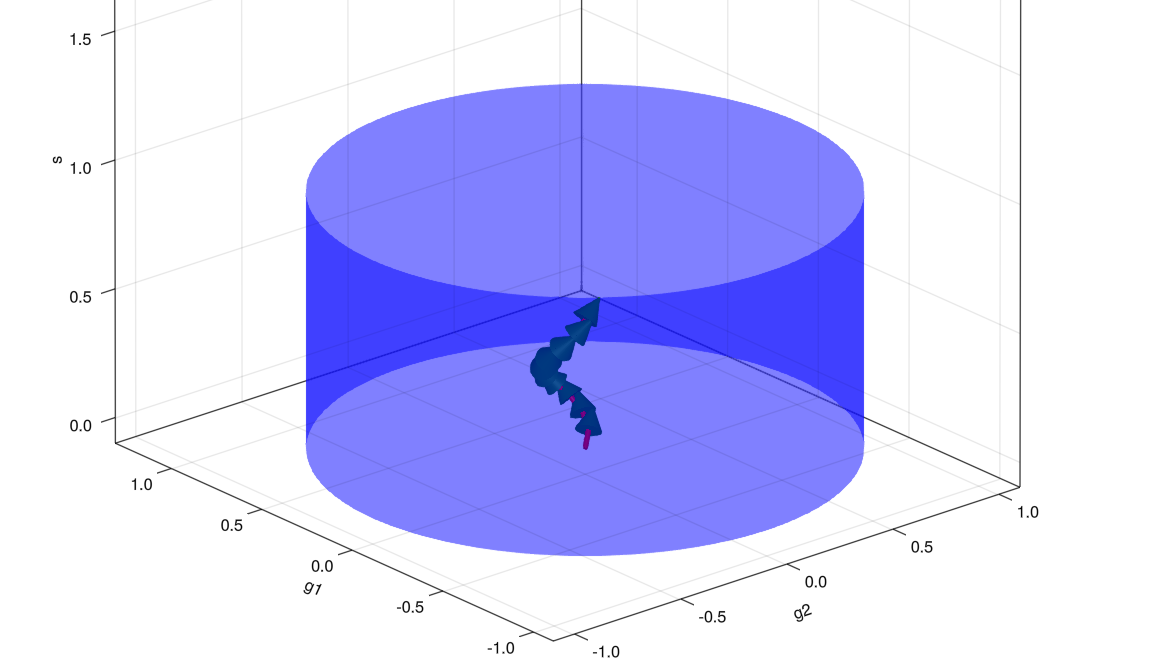
\includegraphics{pathToPoint.png}
\caption{LFBGS algorithm used to find parameters subject to the
cylindrical constraint. s is arbitrarily capped at 1 as a data cleaning
method.}
\end{figure}

\hypertarget{pixel-grid-mode}{%
\subsection{Pixel grid mode}\label{pixel-grid-mode}}

\texttt{ShOpt.jl} provides two modes for pixel grid fits,
\texttt{PCA\ mode} and \texttt{Autoencoder\ mode}. \texttt{PCA\ mode},
outlined below, reconstructs its images using the first \(n\) principal
components. \texttt{Autoencoder\ mode} uses a neural network to
reconstruct the image from a lower dimensional latent space. The network
code written with \texttt{Flux.jl} is also outlined below (Innes 2018).
Both modes provide the end user with tunable parameters that allow for
both perfect reconstruction of star cutouts and low dimensional
representations. The advantage of these modes is that they provide good
reconstructions of the distorted images that can learn the key features
of the point spread function without overfitting the background noise.
In this way it generates a datapoint for our algorithm to train on and
denoises the image in one step. In both cases, the input star data is
cleaned by first fitting an analytic (Gaussian) PSF profile and
rejecting size outliers.

\hypertarget{pixel-methods}{%
\subsubsection{Pixel methods}\label{pixel-methods}}

\texttt{PCA\ mode}

\begin{Shaded}
\begin{Highlighting}[]
\KeywordTok{function}\NormalTok{ pca\_image(image}\OperatorTok{,}\NormalTok{ ncomponents)    }
  \CommentTok{\#Load img Matrix}
\NormalTok{  img\_matrix }\OperatorTok{=}\NormalTok{ image}

  \CommentTok{\# Perform PCA    }
\NormalTok{  M }\OperatorTok{=}\NormalTok{ fit(PCA}\OperatorTok{,}\NormalTok{ img\_matrix}\OperatorTok{;}\NormalTok{ maxoutdim}\OperatorTok{=}\NormalTok{ncomponents)    }

  \CommentTok{\# Transform the image into the PCA space    }
\NormalTok{  transformed }\OperatorTok{=}\NormalTok{ MultivariateStats.transform(M}\OperatorTok{,}\NormalTok{ img\_matrix)    }

  \CommentTok{\# Reconstruct the image    }
\NormalTok{  reconstructed }\OperatorTok{=}\NormalTok{ reconstruct(M}\OperatorTok{,}\NormalTok{ transformed)    }

  \CommentTok{\# Reshape the image back to its original shape    }
\NormalTok{  reconstructed\_image }\OperatorTok{=}\NormalTok{ reshape(reconstructed}\OperatorTok{,}\NormalTok{ size(img\_matrix)}\OperatorTok{...}\NormalTok{)    }
\KeywordTok{end}    
\end{Highlighting}
\end{Shaded}

\texttt{Autoencoder\ mode}

\begin{Shaded}
\begin{Highlighting}[]
\CommentTok{\# Encoder    }
\NormalTok{encoder }\OperatorTok{=}\NormalTok{ Chain(    }
\NormalTok{                Dense(r}\OperatorTok{*}\NormalTok{c}\OperatorTok{,} \FloatTok{128}\OperatorTok{,}\NormalTok{ leakyrelu)}\OperatorTok{,}    
\NormalTok{                Dense(}\FloatTok{128}\OperatorTok{,} \FloatTok{64}\OperatorTok{,}\NormalTok{ leakyrelu)}\OperatorTok{,}    
\NormalTok{                Dense(}\FloatTok{64}\OperatorTok{,} \FloatTok{32}\OperatorTok{,}\NormalTok{ leakyrelu)}\OperatorTok{,}    
\NormalTok{               )    }
\CommentTok{\#Decoder}
\NormalTok{decoder }\OperatorTok{=}\NormalTok{ Chain(    }
\NormalTok{                Dense(}\FloatTok{32}\OperatorTok{,} \FloatTok{64}\OperatorTok{,}\NormalTok{ leakyrelu)}\OperatorTok{,}    
\NormalTok{                Dense(}\FloatTok{64}\OperatorTok{,} \FloatTok{128}\OperatorTok{,}\NormalTok{ leakyrelu)}\OperatorTok{,}    
\NormalTok{                Dense(}\FloatTok{128}\OperatorTok{,}\NormalTok{ r}\OperatorTok{*}\NormalTok{c}\OperatorTok{,}\NormalTok{ tanh)}\OperatorTok{,}    
\NormalTok{               )    }
\CommentTok{\#Full autoencoder}
\NormalTok{autoencoder }\OperatorTok{=}\NormalTok{ Chain(encoder}\OperatorTok{,}\NormalTok{ decoder)    }

\CommentTok{\#x\_hat = autoencoder(x)    }
\NormalTok{loss(x) }\OperatorTok{=}\NormalTok{ mse(autoencoder(x)}\OperatorTok{,}\NormalTok{ x)    }

\CommentTok{\# Define the optimizer    }
\NormalTok{optimizer }\OperatorTok{=}\NormalTok{ ADAM()    }
\end{Highlighting}
\end{Shaded}

\hypertarget{statement-of-need}{%
\section{Statement of need}\label{statement-of-need}}

We can trace the first empirical PSF fitters back to DAOPHOT (Stetson
1987). \texttt{PSFex} made major advancements in precise PSF modeling.
With \texttt{PSFex}, you could interpolate several different bases,
including a basis of pixels, instead of relying on simple parametric
functions. \texttt{PSFex} was built as a general purpose tool and to
this day is widely used. Newer empirical PSF fitters are geared toward
large scale surveys and the difficulties that arise specific to those
datasets. As an example, The Dark Energy Survey and DESCam (Jarvis et
al. 2020; Flaugher et al. 2015) sparked the creation of \texttt{PIFF}.
The recent data from the James Webb Space Telescope poses new
challenges.

\begin{enumerate}
\def\labelenumi{(\arabic{enumi})}
\item
  The JWST PSFs are not well approximated by analytic profiles as seen
  in Figure 1. This calls for well thought out parametric free models
  that can capture the full dynamic range of the Point Spread Function
  without fixating on the noise in the background. Previously, Rowe
  statistics and other parametic equations were used to diagnose PSF
  accurarcy (Rowe 2010). \texttt{ShOpt} provides a suite of parametric
  free summary statistics out of the box.
\item
  The NIRCam detectors are 0.03``/pix or 0.06'' /pix (Rieke et al. 2003;
  Beichman et al. 2012; Rieke, Kelly, and Horner 2005). To capture an
  accurate description of the point spread function at this scale we
  need images that are \(131\) by \(131\) to \(261\) by \(261\) pixels
  across. These vignet sizes are much larger in comparison to the sizes
  needed for previous large surveys such as DES (Jarvis et al. 2020) and
  SuperBIT (McCleary et al. 2023) and forces us to evaluate how well
  existing PSF fitters scale to this size. The DES and SuperBIT surveys
  needed PSF sizes of \(17\) by \(17\) and \(48\) by \(48\), an order of
  magnitude less than the JWST PSF sizes.
\end{enumerate}

\hypertarget{state-of-the-field}{%
\section{State of the Field}\label{state-of-the-field}}

There are several existing empirical PSF fitters in addition to a
forward model of the JWST PSFs developed by STScI (Jarvis et al. 2020 ;
Bertin 2011; Perrin et al. 2014 , 2012). We describe them here and draw
attention to their strengths and weaknesses to motivate the development
of \texttt{ShOpt.jl}. As described in the statement of need,
\texttt{PSFex} was one of the first precise and general purpose tools
used for empirical PSF fitting. However, \texttt{PSFex} produced a
systematic size bias of the point spread function with how it calculated
spatial variation across the field of view (Jarvis et al. 2020). It was
discovered via the analytic profile fits that the size of the point
spread function, governed by the variable \([s]\), was underestimated.

\texttt{PIFF} (Point Spread Functions in the Full Field of View)
followed \texttt{PSFex} in the effort to correct this issue. The DES
camera was \(2.2\) degrees across, which was large enough for the size
bias to become noticable for their efforts. \texttt{PIFF} works in focal
plane coordinates as opposed to pixel coordinates which fixes the
systematic size bias. Jarvis and DES also used the \texttt{Python}
libraries of astropy (Astropy Collaboration et al. 2022) and Galsim
(Rowe et al. 2015) to make the software more accessible than PSFex to
programmers in the astrophysics community. PSFex was written in
\texttt{C} and has been active for more than 20 years. Due to being so
old and written in a low level language it is much less approachable for
a community of open source developers. One of the motivations of
\texttt{ShOpt} was to write astrophysics specific software in
\texttt{Julia}, because \texttt{Julia} provides a nice balance of
readability and speed with it's high level functional paradigm and just
in time compiler. \texttt{ShOpt} works directly in sky coordinates,
which minimizes any bias that might be introduced by transformation from
pixel to sky coordinates afterwords.

While we do have forwards models of the JWST PSF, these models are for
single exposure images. The JWST images are either single exposure or
mosaics (Perrin et al. 2014, 2012). Mosaiced images are essentially
single exposure detector images averaged together. To account for the
rotation of the camera between the capture of images and the wide field
of view, there are a number of steps that make applying these forward
models to mosaics a non trivial procedure. There is also some recent
work being done to generate hybrid models for single exposure data (Lin
et al. 2023). Hybrid models take these forward models and add an
empirical correction. At present, there is yet to be any widely
available software to do this.

The COMOS-Web survey is the largest JWST extragalactic survey according
to area and prime time allocation (Casey et al. 2023), and takes up
\(0.54 ~deg^2\) (Beichman et al. 2012; Rieke et al. 2023). This is a
large enough portion of the sky that we should prepare to see a lot of
variation across the field of view. This gives \texttt{ShOpt} the
oppurtunity to validate PIFF's correction for handling PSF variations
and test how impactful (or not impactful) PSFex's size bias is.

\hypertarget{future-work}{%
\section{Future Work}\label{future-work}}

We speculate that petal diagrams may be able to approximate the spikey
natures of JWST PSFS. Consider \(r = A \cos(k\theta + \gamma)\), shown
below in figure 3 for different \([A, k]\) values where \(\gamma = 0\).
In practice, \([A, k, \gamma]\) could be learnable parameters. Moreover,
we could do this for a series of trigonmetric functions to get petals of
different sizes. We could then choose some \(f(r) \propto \frac{1}{r}\)
such that the gray fades from black to white. We would define \(f(r)\)
piece wise such that it is \(0\) outside of the petal and decreases
radially with \(r\) inside the petal.

\begin{figure}
\centering
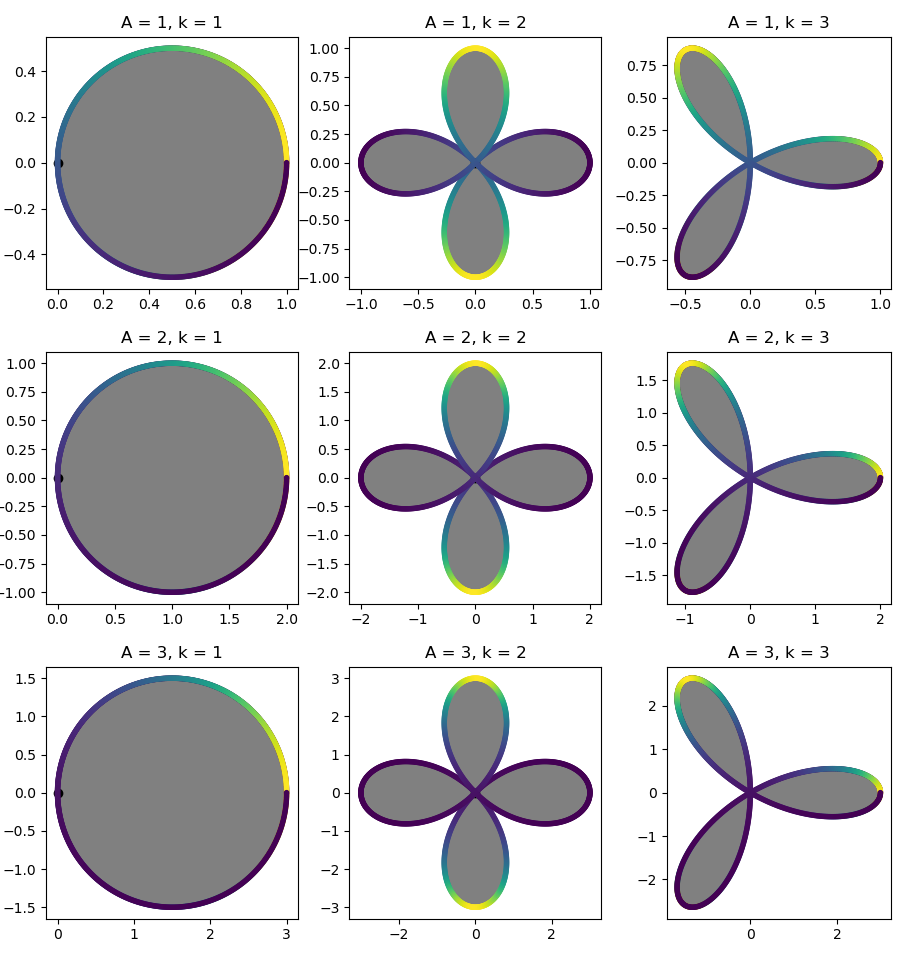
\includegraphics{petals.png}
\caption{Petal Diagram}
\end{figure}

\hypertarget{acknowledgements}{%
\section{Acknowledgements}\label{acknowledgements}}

This material is based upon work supported by a Northeastern University
Undergraduate Research and Fellowships PEAK Experiences Award. We would
also like to thank the Northeastern Physics Department for making this
project possible through the Physics Co-op Research Fellowship. Support
for COSMOS-Web was provided by NASA through grant JWST-GO-01727 and
HST-AR-15802 awarded by the Space Telescope Science Institute, which is
operated by the Association of Universities for Research in Astronomy,
Inc., under NASA contract NAS 5-26555. This work was made possible by
utilizing the CANDIDE cluster at the Institut d'Astrophysique de Paris.
Finally, we would like to thank Northeastern Research Computing for
access to their servers. Additionally, we'd like to extend a thank you
to Professor David Rosen for giving some valuable insights during the
early stages of this work.

\hypertarget{references}{%
\section*{References}\label{references}}
\addcontentsline{toc}{section}{References}

\hypertarget{refs}{}
\begin{cslreferences}
\leavevmode\hypertarget{ref-AbsMahSep2008}{}%
Absil, P.-A., R. Mahony, and R. Sepulchre. 2008. \emph{Optimization
Algorithms on Matrix Manifolds}. Princeton, NJ: Princeton University
Press.

\leavevmode\hypertarget{ref-2022ApJ}{}%
Astropy Collaboration, Adrian M. Price-Whelan, Pey Lian Lim, Nicholas
Earl, Nathaniel Starkman, Larry Bradley, David L. Shupe, et al. 2022.
``The Astropy Project: Sustaining and Growing a Community-oriented
Open-source Project and the Latest Major Release (v5.0) of the Core
Package'' 935 (2): 167. \url{https://doi.org/10.3847/1538-4357/ac7c74}.

\leavevmode\hypertarget{ref-10.1117ux2f12.925447}{}%
Beichman, Charles A., Marcia Rieke, Daniel Eisenstein, Thomas P. Greene,
John Krist, Don McCarthy, Michael Meyer, and John Stansberry. 2012.
``Science opportunities with the near-IR camera (NIRCam) on the James
Webb Space Telescope (JWST).'' In \emph{Space Telescopes and
Instrumentation 2012: Optical, Infrared, and Millimeter Wave}, edited by
Mark C. Clampin, Giovanni G. Fazio, Howard A. MacEwen, and Jacobus M.
Oschmann Jr., 8442:84422N. International Society for Optics; Photonics;
SPIE. \url{https://doi.org/10.1117/12.925447}.

\leavevmode\hypertarget{ref-BSPIE}{}%
Beichman, Charles A., Marcia Rieke, Daniel Eisenstein, Thomas P. Greene,
John Krist, Don McCarthy, Michael Meyer, and John Stansberry. 2012.
``Science opportunities with the near-IR camera (NIRCam) on the James
Webb Space Telescope (JWST).'' In \emph{Space Telescopes and
Instrumentation 2012: Optical, Infrared, and Millimeter Wave}, edited by
Mark C. Clampin, Giovanni G. Fazio, Howard A. MacEwen, and Jr. Oschmann
Jacobus M., 8442:84422N. Society of Photo-Optical Instrumentation
Engineers (Spie) Conference Series.
\url{https://doi.org/10.1117/12.925447}.

\leavevmode\hypertarget{ref-Bergmann2022}{}%
Bergmann, Ronny. 2022. ``Manopt.jl: Optimization on Manifolds in
Julia.'' \emph{Journal of Open Source Software} 7 (70): 3866.
\url{https://doi.org/10.21105/joss.03866}.

\leavevmode\hypertarget{ref-Bernstein_2002}{}%
Bernstein, G. M., and M. Jarvis. 2002. ``Shapes and Shears, Stars and
Smears: Optimal Measurements for Weak Lensing.'' \emph{The Astronomical
Journal} 123 (2): 583. \url{https://doi.org/10.1086/338085}.

\leavevmode\hypertarget{ref-2011ASPC}{}%
Bertin, E. 2011. ``Automated Morphometry with SExtractor and PSFEx.'' In
\emph{Astronomical Data Analysis Software and Systems Xx}, edited by I.
N. Evans, A. Accomazzi, D. J. Mink, and A. H. Rots, 442:435.
Astronomical Society of the Pacific Conference Series.

\leavevmode\hypertarget{ref-boumal2023intromanifolds}{}%
Boumal, Nicolas. 2023. \emph{An Introduction to Optimization on Smooth
Manifolds}. Cambridge University Press.
\url{https://doi.org/10.1017/9781009166164}.

\leavevmode\hypertarget{ref-casey2023cosmosweb}{}%
Casey, Caitlin M., Jeyhan S. Kartaltepe, Nicole E. Drakos, Maximilien
Franco, Santosh Harish, Louise Paquereau, Olivier Ilbert, et al. 2023.
``COSMOS-Web: An Overview of the Jwst Cosmic Origins Survey.''
\url{http://arxiv.org/abs/2211.07865}.

\leavevmode\hypertarget{ref-2015AJ}{}%
Flaugher, B., H. T. Diehl, K. Honscheid, T. M. C. Abbott, and others.
2015. ``The Dark Energy Camera.'' \emph{AJ} 150: 150.
\url{https://doi.org/10.1088/0004-6256/150/5/150}.

\leavevmode\hypertarget{ref-innes:2018}{}%
Innes, Mike. 2018. ``Flux: Elegant Machine Learning with Julia.''
\emph{Journal of Open Source Software}.
\url{https://doi.org/10.21105/joss.00602}.

\leavevmode\hypertarget{ref-Jarvis_2020}{}%
Jarvis, M, G M Bernstein, A Amon, C Davis, P F Lé get, K Bechtol, I
Harrison, et al. 2020. ``Dark Energy Survey Year 3 Results: Point Spread
Function Modelling.'' \emph{Monthly Notices of the Royal Astronomical
Society} 501 (1): 1282--99.
\url{https://doi.org/10.1093/mnras/staa3679}.

\leavevmode\hypertarget{ref-lin2023hybpsf}{}%
Lin, Nie, Huanyuan, Shan, Guoliang, Li, Lei, et al. 2023. ``HybPSF:
Hybrid Psf Reconstruction for the Observed Jwst Nircam Image.''
\url{http://arxiv.org/abs/2308.14065}.

\leavevmode\hypertarget{ref-mccleary2023lensing}{}%
McCleary, Jacqueline E, Spencer W Everett, Mohamed M Shaaban, Ajay S
Gill, Georgios N Vassilakis, Eric M Huff, Richard J Massey, et al. 2023.
``Lensing in the Blue Ii: Estimating the Sensitivity of Stratospheric
Balloons to Weak Gravitational Lensing.'' \emph{arXiv Preprint
arXiv:2307.03295}.

\leavevmode\hypertarget{ref-Mogensen2018}{}%
Mogensen, Patrick K., and Asbjørn N. Riseth. 2018. ``Optim: A
Mathematical Optimization Package for Julia.'' \emph{Journal of Open
Source Software} 3 (24): 615. \url{https://doi.org/10.21105/joss.00615}.

\leavevmode\hypertarget{ref-2014SPIE}{}%
Perrin, Marshall D., Anand Sivaramakrishnan, Charles-Philippe Lajoie,
Erin Elliott, Laurent Pueyo, Swara Ravindranath, and Loic. Albert. 2014.
``Updated point spread function simulations for JWST with WebbPSF.'' In
\emph{Space Telescopes and Instrumentation 2014: Optical, Infrared, and
Millimeter Wave}, edited by Jr. Oschmann Jacobus M., Mark Clampin,
Giovanni G. Fazio, and Howard A. MacEwen, 9143:91433X. Society of
Photo-Optical Instrumentation Engineers (Spie) Conference Series.
\url{https://doi.org/10.1117/12.2056689}.

\leavevmode\hypertarget{ref-2012SPIE}{}%
Perrin, Marshall D., Rémi Soummer, Erin M. Elliott, Matthew D. Lallo,
and Anand Sivaramakrishnan. 2012. ``Simulating point spread functions
for the James Webb Space Telescope with WebbPSF.'' In \emph{Space
Telescopes and Instrumentation 2012: Optical, Infrared, and Millimeter
Wave}, edited by Mark C. Clampin, Giovanni G. Fazio, Howard A. MacEwen,
and Jr. Oschmann Jacobus M., 8442:84423D. Society of Photo-Optical
Instrumentation Engineers (Spie) Conference Series.
\url{https://doi.org/10.1117/12.925230}.

\leavevmode\hypertarget{ref-RevelsLubinPapamarkou2016}{}%
Revels, J., M. Lubin, and T. Papamarkou. 2016. ``Forward-Mode Automatic
Differentiation in Julia.'' \emph{arXiv:1607.07892 {[}cs.MS{]}}.
\url{https://arxiv.org/abs/1607.07892}.

\leavevmode\hypertarget{ref-10.1117ux2f12.489103}{}%
Rieke, Marcia J., Stefi Alison Baum, Charles A. Beichman, David
Crampton, Rene Doyon, Daniel Eisenstein, Thomas P. Greene, et al. 2003.
``NGST NIRCam scientific program and design concept.'' In \emph{IR Space
Telescopes and Instruments}, edited by John C. Mather, 4850:478--85.
International Society for Optics; Photonics; SPIE.
\url{https://doi.org/10.1117/12.489103}.

\leavevmode\hypertarget{ref-20052005SPIE}{}%
Rieke, Marcia J., Douglas Kelly, and Scott Horner. 2005. ``Overview of
James Webb Space Telescope and NIRCam's Role.'' In \emph{Cryogenic
Optical Systems and Instruments Xi}, edited by James B. Heaney and
Lawrence G. Burriesci, 5904:1--8. Society of Photo-Optical
Instrumentation Engineers (Spie) Conference Series.
\url{https://doi.org/10.1117/12.615554}.

\leavevmode\hypertarget{ref-Rieke_2023}{}%
Rieke, Marcia J., Douglas M. Kelly, Karl Misselt, John Stansberry,
Martha Boyer, Thomas Beatty, Eiichi Egami, et al. 2023. ``Performance of
Nircam on Jwst in Flight.'' \emph{Publications of the Astronomical
Society of the Pacific} 135 (1044): 028001.
\url{https://doi.org/10.1088/1538-3873/acac53}.

\leavevmode\hypertarget{ref-doi:10.1177ux2f0278364918784361}{}%
Rosen, David M, Luca Carlone, Afonso S Bandeira, and John J Leonard.
2019. ``SE-Sync: A Certifiably Correct Algorithm for Synchronization
over the Special Euclidean Group.'' \emph{The International Journal of
Robotics Research} 38 (2-3): 95--125.
\url{https://doi.org/10.1177/0278364918784361}.

\leavevmode\hypertarget{ref-Barnaby2010MNRAS}{}%
Rowe, Barnaby. 2010. ``Improving PSF modelling for weak gravitational
lensing using new methods in model selection'' 404 (1): 350--66.
\url{https://doi.org/10.1111/j.1365-2966.2010.16277.x}.

\leavevmode\hypertarget{ref-rowe2015galsim}{}%
Rowe, Barnaby, Mike Jarvis, Rachel Mandelbaum, Gary M. Bernstein, James
Bosch, Melanie Simet, Joshua E. Meyers, et al. 2015. ``GalSim: The
Modular Galaxy Image Simulation Toolkit.''
\url{http://arxiv.org/abs/1407.7676}.

\leavevmode\hypertarget{ref-Stetson_1987}{}%
Stetson, Peter B. 1987. ``DAOPHOT: A Computer Program for Crowded-Field
Stellar Photometry.'' \emph{Publications of the Astronomical Society of
the Pacific} 99 (613): 191. \url{https://doi.org/10.1086/131977}.
\end{cslreferences}

\end{document}
